\chapter{Разработка пользовательского интерфейса}

Описав основные документы, которые необходимо заполнить при предоставлении услуги,
нам требуется описать, как они будут заполнятся.

К счастью, в Bizagi Studio есть полноценный редактор форм, с помощь которого
можно создать необходимые формы в несколько кликов мыши.

\myImage{Перейдя в <<Define Forms>>, нам нужно выбрать для какого
действия нужно создать формы (помечены восклицательным знаком)}{50-add-form}{50-add-form}
\myImage{Перетаскивая аттрибуты данных на форму,
можем легко сформировать панель для регистрации инструментов
(Красным подсвечены поля обязательные для заполнения на данном этапе)
}{50-register-form}{50-register-form}
\myImage{Отправка запроса в ИЦ - не может быть автоматизирвоана по внешним причинам,
поэтому просто дадим исполнителю необходимую информацию и добавим подтверждение
об отправке заявления в ИЦ}{50-request}{50-request}

\myImage{Внесение сведений о судимости в модель.
На этом этапе остальные поля уже не меняются}{50-journal}{50-journal}
\begin{figure}[!ht]
    \centering
    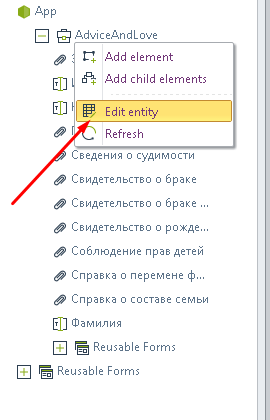
\includegraphics[width=0.5\textwidth]{figures/50-edit}
    \caption{При необходимости, можно отредактировать модель прямо в редакторе форм}
    \label{50-edit}
\end{figure}